%% ++++++++++++++++++++++++++++++++++++++++++++++++++++++++++++
%% Hauptdatei, Wurzel des Dokuments
%% ++++++++++++++++++++++++++++++++++++++++++++++++++++++++++++
%
%  Gerüst:
%   * Version 1.00
% 	* erstellt von: Samir Charif
% 	* Mai 2022
% 	* Mail: s.charif@tu-braunschweg.de
% !TeX program = lualatex


%% Import der Formatierung
% only change this if you know what you do!!!
%  Instalation der Pakete: 
%  * Version 1.0
%  * Samir Charif
%  * s.charif@tu-braunschweig.de
%  * Student, TU Braunschweig
%  * Mai 2022
%
%  Für Hauptseminare, Studienarbeiten, Diplomarbeiten
%
%  Autor           : Max Mustermann
%  Letzte Änderung : Morgen
%
\newcommand\myBCOR{17mm}

\documentclass
[   twoside=false,     % Einseitiger oder zweiseitiger Druck?
twocolumn=false,%			zweispaltiger Satz
fontsize=12pt,     % Bezug: 12-Punkt Schriftgröße
DIV=15,            % Randaufteilung, siehe Dokumentation "KOMA"-Script
BCOR=\myBCOR,         % Bindekorrektur: Innen 17mm Platz lassen. Copyshop-getestet.
%    headsepline,
headsepline=true,  % Unter Kopfzeile Trennlinie (aus: headnosepline)
footsepline=true,  % Über Fußzeile Trennlinie (aus: footnosepline)
open=right,        % Neue Kapitel im zweiseitigen Druck rechts beginnen lassen
paper=a4,          % Seitenformat A4
chapterentrydots=true,%	Inhaltsverzeichnis dotfill für Kapitel
chapterprefix=false,%		Kapitelprefix für mainmatter
appendixprefix=false,%		Kapitelprefix für Anhang
abstract=true,     % Abstract einbinden
listof=totoc,      % Div. Verzeichnisse ins Inhaltsverzeichnis aufnehmen
bibliography=totoc,% Literaturverzeichnis ins Inhaltsverzeichnis aufnehmen
%bibliography=oldstyle,%		Formatierungsstil des Literaturverzeichnisses %openstyle
titlepage=true,         % Titelseite aktivieren
headinclude=true,  % Seiten-Head in die Satzspiegelberechnung mit einbeziehen
footinclude=false, % Seiten-Foot nicht in die Satzspiegelberechnung mit einbeziehen
numbers=noenddot,   % Gliederungsnummern ohne abschließenden Punkt darstellen
index=default,%				Index im Inhaltsverzeichnis %totoc %numbered
DIV = 15,		%Type area settings (See KOMA-Script p.36) DIV-Wert fuer die Erstellung des Satzspiegels, siehe scrguide	%calc
%parskip=false,%				Der erste Absatz eines Abschnitts wird nicht eingezogen
%parskip=half,%				Absatzabstand statt Absatzeinzug
captions=tableheading, %
draft=false,%				Keine Bilder in der Anzeige, overfull hboxes werden angezeigt
greek, english, ngerman %Languages the last one decides about the automatically created text
]   {scrreprt}         % Dokumentenstil: "Report" aus dem KOMA-Skript-Paket

%\usepackage[first,light]{draftcopy} % Für Probedruck

%% ++++++++++++++++++++++++++++++++++++++++++++++++++++++++++++
%% Handling
%% ++++++++++++++++++++++++++++++++++++++++++++++++++++++++++++

\usepackage{ifthen}		% 

\usepackage{verbatim}  % Mehrzeilige Kommentare ohne % vor jeder Zeile. 
%\begin{verbatim}
%Leider funktioniert es nicht so, dass eine verbatim Umgebung
%einfach in eine andere geschrieben werden kann. Stattdessen kommt
%der Befehl \verb+Irgendwas+ zum Einsatz um den Quellecode zu zeigen.
%\end{verbatim}
%\begin{comment}
%Der Text der innerhalb der \emph{comment} Umgebung steht 
%wird nicht ausgegeben und es werden auch keine Befehle 
%abgearbeitet.
%\end{comment}


% Für TU BS
\usepackage{scrhack}
\usepackage{ifluatex}
\ifluatex \else \usepackage{scrwfile} \fi		% Verbindet Befehle und führt die aus
\usepackage{etoolbox}		%  


\usepackage{scrhack} 		% scrhack redefines macros of packages


%% ++++++++++++++++++++++++++++++++++++++++++++++++++++++++++++
%% Sprachen, Text und Eingabekodierung
%% ++++++++++++++++++++++++++++++++++++++++++++++++++++++++++++

\usepackage[english, main=ngerman, headfoot=ngerman]{babel}   % Sprachpakete / Worttrennung / die letzte Sprache wird als Standart ausgewählt
\usepackage{textgreek} 		   % griechische Buchstaben im Text

%\usepackage[T1]{fontenc} 	  % Festlegen der Schriftart / Option T1
%\usepackage[latin1]{inputenc} % Zeichencodierung nach ISO-8859-1
%ermöglicht das Verwenden von Umlauten  (Westeuropa)  Umlaute für Westeuroüa
\ifluatex
	\usepackage[utf8]{luainputenc}%				Nötig um Umlaute zu tippen. Alternativ: latin1
\else
	\usepackage[utf8]{inputenc}   %	Zeichencodierung nach UTF-8 (Unicode) / 
\fi

\ifluatex
%% if using luatex and not using latexmk, this can be use for executing bib2gls
\directlua{local t = os.execute("bib2gls --tex-encoding UTF-8 --group " .. status.filename:sub(1, -5))
print(t)
}
\else
\usepackage[T1]{fontenc}%				font encoding
\fi


\usepackage{lmodern}		  % Das lmodern (= Latin Modern) Paket verändert die verwendete Schriftart --> Darstellung erscheint flüssiger




\usepackage[normalem]{ulem}		% Unterstreichen von Absätzen

%\usepackage[autostyle]{csquotes}
\usepackage{csquotes}			% Anführungzeichen an die Sprache angebpasst \enquote{Menu}

% Improved typesetting
%\usepackage[final]{microtype} 
%\usepackage{microtype} 
%		\RequirePackage[all]{nowidow}
%		\DeclareMicrotypeAlias{ }{TU-basic}
\usepackage{textcomp} % Setup microtype and siunitx
\usepackage{xstring}	%String manipulation
\newcommand\IfStringInList[2]{\IfSubStr{,#2,}{,#1,}}	% für das Suchen von Strings in Listen

\usepackage{setspace}


%% ++++++++++++++++++++++++++++++++++++++++++++++++++++++++++++
%% Rand und Formatierung
%% ++++++++++++++++++++++++++++++++++++++++++++++++++++++++++++

%\usepackage[activate=normal]{pdfcprot} 	% Optischer Randausgleich -> pdflatex!
\usepackage{setspace}				   	% Einstellen des Zeilenabstands, Zeilenabstand in Fusßnoten wird nicht gändert. Einstellmöglichkeiten: singlespacing, onehalfspacing, doublespacing

\usepackage[automark]{scrlayer-scrpage} % individuelle Kopf- und Fußzeilen


% Tiefe der Kapitelnummerierung beeinflussen
\setcounter{secnumdepth}{3} % Tiefe der Nummerierung
\setcounter{tocdepth}{2}    % Tiefe des Inhaltsverzeichnisses


%% ++++++++++++++++++++++++++++++++++++++++++++++++++++++++++++
%% Formelzeichen
%% ++++++++++++++++++++++++++++++++++++++++++++++++++++++++++++
%\usepackage[
%nonumberlist, %keine Seitenzahlen anzeigen
%toc,          %Einträge im Inhaltsverzeichnis
%section=chapter]      %im Inhaltsverzeichnis auf section-Ebene erscheinen
%{glossaries}
%%\usepackage{hyperref}



%% ++++++++++++++++++++++++++++++++++++++++++++++++++++++++++++
%% Tabellen
%% ++++++++++++++++++++++++++++++++++++++++++++++++++++++++++++

% \usepackage[table]{xcolor} % Farben in Tabellen
\usepackage{makecell}	   % Alignment der Zellen /Tabellarische Säulenköpfe und mehrzeilige Zellen

%\usepackage{tabularx}		% Tabellarische Übersichten mit einstellbarer Spaltenbreite
%\usepackage{longtable}		% Zulassen, dass Tabellen über Seitengrenzen hinweg fließen
\usepackage{ltxtable}		% longtable + tabularx
\usepackage{multirow}		% Erstellen von Tabellenzellen, die sich über mehrere Zeilen erstrecken
\usepackage{booktabs}		% Tabellenformatierung
%\usepackage[hang, bf, font=small, textformat=period]{caption}%
\usepackage{caption}
\usepackage{subcaption}		% Package um subfigure zu erstellen
\usepackage{colortbl} 		% Support for colors in tables

\usepackage{array,			%
			ragged2e,		%  Alignment der Zellen 
			calc}			% fügt Infix-Ausdrücke hinzu, um die Argumente der LATEX-Befehle arithmetisch zu bearbeiten 
\usepackage{lscape}			% Ausgewälte Bereiche können im Querformat angzeigt werden
\usepackage[flushleft]{threeparttable} % Tabellen mit Beschriftungen und Notizen in gleicher Breite
%%Adjust line thickness
%\setlength{\heavyrulewidth}{0.15em}
%\setlength{\lightrulewidth}{0.05em}
%\setlength{\cmidrulewidth}{0.05em}

%% ++++++++++++++++++++++++++++++++++++++++++++++++++++++++++++
%% Grafiken
%% ++++++++++++++++++++++++++++++++++++++++++++++++++++++++++++
\ifluatex
%	\usepackage[luatex]{graphicx}%			Package um grafiken zu includieren
	\RequirePackage[svgnames, table, luatex]{xcolor}
\else
	\usepackage[pdftex]{graphicx}%
	\RequirePackage[svgnames, table, pdftex]{xcolor}
\fi
\usepackage[svgnames, table]{xcolor}%				Farbkonversion etc.
%\usepackage{graphicx}		% Einbinden von Bildern. 
%				 final: hebt draft auf
%				 draft: anstatt der bilder wird nur ein Kasten angezeigt --> schnelleres kompelieren
% \usepackage{grffile}  % Das Paket erweitert die Dateinamenverarbeitung des Grafikpakets, um einen größeren Bereich von Dateinamen zu unterstützen. Der Dateiname kann zum Beispiel mehrere Punkte enthalten.
\graphicspath{{../Bilder}} % Verzeichnis der Bilder

\usepackage{rotating}		% Rotieren von Bildern Tabellen, ganzen Seiten

%%% Modifications
\usepackage{float}		% Automatische Platzierung von Grafiken im Dokument / https://en.wikibooks.org/wiki/LaTeX/Floats,_Figures_and_s
%\restylefloat{figure}	% Rahmen um Bilder

%\usepackage{subfig}     % Subfigures in einer Figure erstellen

%% Tikz
\usepackage{tikz}
\usepackage{tikzpagenodes} %Defines extra anchors on the page 
\usetikzlibrary{shapes.arrows,arrows,arrows.meta,backgrounds,calc,patterns, 
	shapes.geometric,decorations.pathmorphing,decorations.markings,decorations.text,matrix,fit,intersections}

%\usepackage[tx, RPvoltages]{circuitikz}%		Zeichnen von elektrischen Schaltbildern direkt in Latex


%%% Matlab2tikz
\usepackage{pgfplots}	% PGFPlots zeichnet hochwertige Funktionsdiagramme 
%\pgfplotsset{compat=newest}	% newest = neuste, nicht empfohlen
\pgfplotsset{compat=1.3} % 1.3 Standartwert, empfohlenen Wert aus Logfile suchen
%% the following commands are needed for some matlab2tikz features
\usetikzlibrary{plotmarks}	% Plotmakierungen wie Sterne etc
\usetikzlibrary{arrows, arrows.meta, shapes.geometric}

\usepgfplotslibrary{patchplots}	% Patch-Plots ähneln den Mesh- und Surf-Plots insofern, als sie eine gefüllte Fläche anhand einer Geometrie beschreiben.


\usepackage{pdfpages} 		% Einfügen von PDFs



%% ++++++++++++++++++++++++++++++++++++++++++++++++++++++++++++
%% Verlinkung
%% ++++++++++++++++++++++++++++++++++++++++++++++++++++++++++++

\usepackage[active]{srcltx}		% Dieses Paket bietet eine spezielle Einfügung von Quellen in DVI-Dateien, die es ermöglicht von der DVI-Datei zum .tex-Quelltext und zurück zu springen (vorausgesetzt ein DVI-Viewer der dies unterstützt). Zusätzlich bietet es Hooks für die Fehlerverfolgung aus der .log-Datei für die WinEdt-Shell.

\usepackage[T1]{url}			% Verlinkungen von URLs
%\usepackage{hyperref}			% Verlinkung von URLs und Verweisen
%hyperref wird von pdfcomment geladen 
 
\usepackage[plainpages=false,pdfpagelabels,hypertexnames=false]{hyperref}   % Verlinkung von URLs und Verweisen
			% plainpages: Erzwingt die Benennung von Seitenankern nach der arabischen Form der Seitenzahl benannt werden und nicht nach der formatierten Form.
			% pdfpagelabels: PDF-Seitenbeschriftungen festlegen
			% hypertexnames: benutzt erratbare Namen für Links verwenden

\usepackage{cooltooltips}

%% ++++++++++++++++++++++++++++++++++++++++++++++++++++++++++++
%% Formelen
%% ++++++++++++++++++++++++++++++++++++++++++++++++++++++++++++

\usepackage{amsmath} % Mathe Umgebung
%\usepackage{amsfonts}%				Standard fonts
\usepackage{amssymb}	%	Pfeile Symbole
\usepackage{gensymb}	% 	Einheiten für Text und Mathmode
\usepackage{array}		% Eine erweiterte Implementierung der Array- und Tabellenumgebung, die die Optionen für Spaltenformate erweitert und "programmierbare" Formatspezifikationen bietet
\usepackage{mathtools}%				Multiline and split equations / Formattierung
\usepackage{relsize}	% Änderung der Relativen größe einzelner Symbole in Formeln
\usepackage{mleftright}	% Das Paket definiert Varianten \mleft und \mright von \left und \right, die die Begrenzungszeichen wie \mathopen und \mathclose wirken lassen. Diese Befehle beheben Probleme mit den Abständen in Unterformeln.
	\mleftright%
\ifluatex
\usepackage{lualatex-math}%		patches a few commands of the LaTeX2ε kernel and the amsmath and mathtools packages
\fi

% comprehensive Viele Symbole
%\usepackage{comprehensive}	% 



% Tabellenspaltendefinitionen mit fester Breite --> somit Zeilenumbruch innerhalb einer Zelle möglich
% aus http://www.torsten-schuetze.de/tex/tabsatz-2004.pdf
\usepackage{array, booktabs}
\newcolumntype{f}{>{$}l<{$}}
\newcolumntype{n}{>{\raggedright}l}
\newcolumntype{N}{>{\scriptsize}l}
\newcolumntype{v}[1]{>{\raggedright\hspace{0pt}}m{#1}}
\newcolumntype{V}[1]{>{\scriptsize\raggedright\hspace{0pt}}m{#1}}
\newcolumntype{Z}[1]{>{\raggedright\centering}m{#1}}
\newcolumntype{k}[1]{>{\raggedright}p{#1}}
% ergibt Tabllenspalte fester Breite, linksbündig
% Umbruch innerhalb der Zelle mit \\, neue Tabellezeile mit \tabularnewline
% \addlinespace für Gruppentrennung (aus \texttt{booktabs.sty})


% Einheiten
\usepackage[allow-number-unit-breaks=false, % Kontroliert den Zeilenumbruch zwischen Zahl und Einheit
	range-units=single,		% Bei einer Range wird die Einheit nur hinter der letzten Zahl angezeigt
	list-units = single,	% Bei einer Liste wird die Einheit nur hinter der letzten Zahl angezeigt
	exponent-product = \ensuremath{\cdot}, % Zwischen exponent und Zahl mit Punkt trennen
	separate-uncertainty %Mit der Option separate-uncertainty wird zwischen der Zahl und dem Fehlerterm ein Plusminuszeichen gesetzt.
	]{siunitx}
\sisetup{
	locale = DE,% 	% Stellt das Paket auf deutsch -> Trennzeichen sind Kommas etc.
	detect-all,%
	% 		scientific-notation = engineering,%
	list-final-separator = { und },	
	list-pair-separator = { und },%
	list-units = single,	% Bei Aufzählungen werden in der From 1 bis 7 N dargestellt
	range-phrase = { bis },%	 Bei Aufzählungen werden in der From 1 bis 7 N
	per-mode = symbol,%
	output-complex-root = j,%
}
	% Benutzer derfinierte Einheiten deklarieren
	\DeclareSIUnit[]\dBm{dBm}
	\DeclareSIUnit[]\dBW{dBW}
	\DeclareSIUnit\ions{Ions}
	\DeclareSIUnit\lightyear{ly}  

% Benutzerdefiniert Befehle für SIUnitx
\NewDocumentCommand{\siprefix}{m}{%
	\unit{#1\nonexistentunitjustforprefixes}%
}
\DeclareSIUnit{\nonexistentunitjustforprefixes}{\relax}

% Um Konflikt zwishcen siunitx und physics bezüglich \qty zu vermeiden	
%\let\svqty\qty	
%\usepackage{physics}
%\let\qty\svqty

% Berechnungen in Latex
\usepackage{calc}%							Hilfspaket um mit Latex variablen zu rechnen

%% ++++++++++++++++++++++++++++++++++++++++++++++++++++++++++++
%% Programcode im Text
%% +++++++++++++++++++++++++++++++++++++++++++++++++++++++++++
\usepackage{listings} 	% Ermöglicht das Verwendden con Programcode im Text
%\lstnewenvironment{matlab}[1][]{
%	\lstset{
%		backgroundcolor=\color{white}, %\color{TUgreen!20}, %\color{gray!20}
%		fillcolor=,% %\color{black},
%		captionpos=t,% b
%		tabsize=4,%
%		rulecolor=\color{black},%
%		rulesepcolor=\color{gray!30},%
%		language=Matlab,%
%		basicstyle=\small,%
%		numbers=left,%
%		numberfirstline=true,%
%		numberblanklines=true,%
%		stepnumber=1,%
%		numbersep=5pt,%
%		numberstyle=\scriptsize,%
%		upquote=true,%
%		aboveskip={0\baselineskip},%
%		% 		belowskip=\baselineskip,%
%		columns=flexible,% %fixed,
%		showstringspaces=false,%
%		extendedchars=true,%
%		breaklines=true,%
%		breakatwhitespace=true,%
%		prebreak = \raisebox{0ex}[0ex][0ex]{\ensuremath{\color{black}\hookleftarrow}},%
%		breakautoindent=true,%
%		frame=single,% %tblr, %shadowbox, %tblrTBLR,
%		frameround=ffff,% %tttt,
%		showtabs=false,%
%		showspaces=false,%
%		showstringspaces=false,%
%		identifierstyle=\ttfamily,%
%		basicstyle=\ttfamily\color{black},%
%		keywordstyle=\ttfamily\bfseries\color{MidnightBlue},%
%		commentstyle=\color{tudark},% %\color{MediumTurquoise},
%		stringstyle=\color{DarkOrchid},%
%		mathescape=true,%
%		showlines=true,%
%		escapechar=§,%							escape to latex
%		abovecaptionskip=0\smallskipamount,%
%		belowcaptionskip=3\smallskipamount,%
%		xleftmargin=1.25\baselineskip,%
%		xrightmargin=0pt,
%		#1,%									add more options from the optional parameter
%}}{}
\lstset{numbers=left,stepnumber=2,, numberstyle=\tiny, numbersep=5pt, basicstyle=\small, language=Matlab}	% Einstellungen des liltings Packages
% used Language
% \lstset{language=Matlab}

%% ++++++++++++++++++++++++++++++++++++++++++++++++++++++++++++
%% PDF
%% ++++++++++++++++++++++++++++++++++++++++++++++++++++++++++++

\usepackage{pdfcomment} 	% Ermöglicht das kommentieren in PDF Files

\hypersetup{plainpages=false,hypertexnames=false}

\usepackage{hyperxmp} 		% metadata addon



%% ++++++++++++++++++++++++++++++++++++++++++++++++++++++++++++
%% Verzeichnisse
%% ++++++++++++++++++++++++++++++++++++++++++++++++++++++++++++
\usepackage{scrhack}		% Entfernt Fehler von nym der durch Verwendung alter Biliotheken entsteht.
%\usepackage[printonlyused,nohyperlinks]{acronym} % Abkürzungsverzeichnis
		% footnote: Bei der Verwendung der Option footnote wird die Langform der Abkürzung als Fußnote in das Dokument eingefügt.
		% nohyperlinks: Die Option nohyperlinks wird die Verlinkung der Abkürzung, bei gleichzeitiger Verwendung des hyperref Paktes verhindert.
		% printonlyused: Mit der Option printonlyused werden nur die Abkürzungen ausgegeben, die auch innerhalb des Dokumentes verwendet worden sind. Wird diese Option verwendet kann auch die Option withpage genutzt werden, sie dient dazu die entsprechende Seitenzahl anzuzeigen.
		% smaller: Die Option smaller verkleinert die Anzeige der Abkürzung im Dokument.
		% dua: Wird die Option dua gesetzt, wird immer die Langform der Abkürzung angezeigt. Es sei denn es wurden die Kurzform Befehle wie etwa \acs{Kuerzel} oder \acsp{Kuerzel} verwendet. In diesen Fällen wird dann auch bei der gesetzten Option dua die Kurzform im Dokument dargesetellt.
		% nolist: Die Option nolist führt dazu, dass keine Übersicht von den Abkürzungen erstellt wird.

		% Eigener Plural möglich

		
%% Textbefehle für das glostools Package
\newcommand{\markup}[1]{\textbf{#1}}	% Fettschreiben

%% -- glostools --> Nomenkaltur 
\usepackage[qtmarkupright,	% define char <"> as shortcut for "sbu" macro in math mode  and define qtmark macro to show the quotation mark character
	singlelineskip,	% zeilenabstand im Verzeichnis für größeren Abstand auskommentieren
	 toc]{glosmathtools}
% Hier eintragen welche Listen mit Einheit angezeigt werden sollen.
% Möglichkeiten: latin,greek,vecMat,subscript,operator,abbrv -> keine Leerzeichen!
\newcommand{\miteinheit}{latin,greek}
\usepackage{Formatierung/glosstyle}
%% ---------- nomenclature base style ----------------------------------------
%\newcounter{glosmath@mainEntryCtr}% 
%\newlength{\glosmath@curNameLen}%	
%\newcommand*{\glosstyledesc}[1]{}%
% Hier eintragen welche Listen mit Einheit angezeigt werden sollen.
% Möglichkeiten: latin, greek, vecMat, subscript, operator, abbrv
\newcommand{\miteinheit}{latin, greek, vecMat}

\renewglossarystyle{glosmath@glostyle}%
{%
	\setglossarystyle{alttree}% based on alttree style
	\renewenvironment{theglossary}%
	{%
		\let\glosmath@oldparskip\parskip%
		\setlength{\parskip}{0pt}%
		\let\glosmath@oldparindent\parindent%
		\setlength{\parindent}{0pt}%
	}%
	{%
		\setlength{\parskip}{\glosmath@oldparskip}%
		\setlength{\parindent}{\glosmath@oldparindent}%
	}%
	\renewcommand*{\glossaryheader}%
	{%
		\iftoggle{glosmath@singlelineskip}{%
			\ifdefined\SingleSpacing\SingleSpacing\fi% memoir class
			\ifdefined\singlespacing\singlespacing\fi% setspace package
		}{}%
	}%
	\setcounter{glosmath@mainEntryCtr}{0}%
	\setlength{\glosmath@curNameLen}{\glstreeindent}%
	% desc in all languages of the style (default to main language only) :
	\renewcommand*{\glosstyledesc}[1]{\glsentrydesc{##1}}%
	\renewcommand*{\glossentry}[2]%
	{%
		\ifnum\value{glosmath@mainEntryCtr}>0\vspace{\baselineskip}\fi%
		\glstarget{##1}{\glscatnamefmt{\glosstyledesc{##1}}}%
		\par\nopagebreak%
		\stepcounter{glosmath@mainEntryCtr}%
	}%
	\renewcommand*{\subglossentry}[3] {%
		\IfStringInList{\glsentryparent{##2}}{\miteinheit}{%		Wenn parent = latin 
			\settowidth{\glstreeindent}{\@glswidestname\glstreepredesc}%
			\hangindent\glstreeindent%
			\settowidth{\glosmath@curNameLen}{\glossentryname{##2}\glstreepredesc}%
			% larger namebox for entries longer than @glswidestname :
			\ifdimgreater{\glosmath@curNameLen}{\glstreeindent}{%
				\setlength{\glstreeindent}{\glosmath@curNameLen}}{}%
			\glstreenamebox{\glstreeindent}{%
				\glstarget{##2}{\glossentryname{##2}}%
			}%
			\ifglshassymbol{##2}{
				\settowidth{\glstreeindent}{\@glswidestname\glstreepredesc}%
				\hangindent\glstreeindent%
				\settowidth{\glosmath@curNameLen}{\glossentrysymbol{##2}\glstreepredesc}%
				% larger namebox for entries longer than @glswidestname :
				\ifdimgreater{\glosmath@curNameLen}{\glstreeindent}{%
					\setlength{\glstreeindent}{\glosmath@curNameLen}}{}%
				\glstreenamebox{\glstreeindent}{%
					\glstarget{##2}{\glossentrysymbol{##2}}%
				}%
			}{
				\settowidth{\glstreeindent}{\@glswidestname\glstreepredesc}%
				\hangindent\glstreeindent%
				\settowidth{\glosmath@curNameLen}{\glstreepredesc}%
				% larger namebox for entries longer than @glswidestname :
				\ifdimgreater{\glosmath@curNameLen}{\glstreeindent}{%
					\setlength{\glstreeindent}{\glosmath@curNameLen}}{}%
				\glstreenamebox{\glstreeindent}{%
					\glstarget{##2}{}%
				}%
			}
			%		\ifglshassymbol{##2}{\glossentrysymbol{##2} ,\space}{}%
			\glosstyledesc{##2}%
			
			\par%
		}%
		{% else
			\settowidth{\glstreeindent}{\@glswidestname\glstreepredesc}%
			\hangindent\glstreeindent%
			\settowidth{\glosmath@curNameLen}{\glossentryname{##2}\glstreepredesc}%
			% larger namebox for entries longer than @glswidestname :
			\ifdimgreater{\glosmath@curNameLen}{\glstreeindent}{%
				\setlength{\glstreeindent}{\glosmath@curNameLen}}{}%
			\glstreenamebox{\glstreeindent}{%
				\glstarget{##2}{\glossentryname{##2}}%
			}%
			\glosstyledesc{##2}%
			
			\par%
		}%
	}%
}%


\makeglossaries% executed in first
\setacronymlang{L1}% first language abbreviations
\setglossarystyle{nomencl-L1}% bilingual description
\loadglsentries{Kapitel/sample_glosmathtools_glos} % definition file
\glssetwidest{LOOP}  % IMPORTANT : widest entry in nomenclature



%% ++++++++++++++++++++++++++++++++++++++++++++++++++++++++++++
%% Seitenlayout und Kapitel Formatierung
%% ++++++++++++++++++++++++++++++++++++++++++++++++++++++++++++


% Seitenlayout festlegen. Hier nichts ändern!
\pagestyle{scrplain}
\ihead[]{\headmark}
\ohead[]{\pagemark}
\chead[]{}
\ifoot[]{}
\ofoot[]{\scriptsize \artderausarbeitung\ \namedesautors}
\cfoot[]{}
\renewcommand{\titlepagestyle}{scrheadings}
\renewcommand{\partpagestyle}{scrheadings}
\renewcommand{\chapterpagestyle}{scrheadings}
\renewcommand{\indexpagestyle}{scrheadings}

% Abschnittsweise Nummerierung anstatt fortlaufend. Hier nichts ändern!
\makeatletter
\@addtoreset{equation}{chapter}
\@addtoreset{figure}{chapter}
\@addtoreset{table}{chapter}
\renewcommand\theequation{\thechapter.\@arabic\c@equation}
\renewcommand\thefigure{\thechapter.\@arabic\c@figure}
\renewcommand\thetable{\thechapter.\@arabic\c@table}
\makeatother

% Quelltextrahmen, klein. Hier nichts ändern!
\newsavebox{\inhaltkl}
\def\rahmenkl{\sbox{\inhaltkl}\bgroup\small\renewcommand{\baselinestretch}{1}\vbox\bgroup\hsize\textwidth}
\def\endrahmenkl{\par\vskip-\lastskip\egroup\egroup\fboxsep3mm%
	\framebox[\textwidth][l]{\usebox{\inhaltkl}}}

% Quelltextrahmen, normale Groesse. Hier nichts ändern!
\newsavebox{\inhalt}
\def\rahmen{\sbox{\inhalt}\bgroup\renewcommand{\baselinestretch}{1}\vbox\bgroup\hsize\textwidth}
\def\endrahmen{\par\vskip-\lastskip\egroup\egroup\fboxsep3mm%
	\framebox[\textwidth][l]{\usebox{\inhalt}}}
%




%% ++++++++++++++++++++++++++++++++++++++++++++++++++++++++++++
%% Literaturverzeichnis
%% ++++++++++++++++++++++++++++++++++++++++++++++++++++++++++++
%\usepackage[style=ieee, backend=bibtex]{biblatex}
%\addbibresource{literatur}


\usepackage[
backend=biber,
%style=numeric, %alphabetic
style=ieee,
sortlocale=de_DE,
natbib=true,
url=false, 
doi=false,
eprint=false,
isbn=false,
giveninits=true,
minbibnames=1,
maxbibnames=2
]{biblatex}

%Supression of the note field
\AtEveryBibitem{%
	\clearfield{note}%
}

%%% ++++++++++++++++++++++++++++++++++++++++++++++++++++++++++++
%%% TU Braunschweig Schriftart und Fraben
%%% ++++++++++++++++++++++++++++++++++++++++++++++++++++++++++++
\usepackage{tubscolors}
\usepackage{tubslogo}

%%\usepackage{fontspec}
%%\setmainfont{NexusSerifPro}[%
%%Path = ./fonts/otf/,%
%%Extension = .otf,%
%%UprightFont = *-Regular,%
%%BoldFont = *-Bold]%
%%
%%\setsansfont{NexusSansPro}[%
%%Path = ./fonts/otf/,%
%%Extension = .otf,%
%%UprightFont = *-Regular,%
%%BoldFont = *-Bold]%
%
%


% change this for individual style of table and flowchartstyle
%\input{Formatierung/appearance.tex}

% Eigene Farben
%  Farben:
%  * Version 1.0
%  * Samir charif
%  * Student, TU Braunschweig
%  * Mai 2022
%
%  Für Hauptseminare, Studienarbeiten, Diplomarbeiten
%
%  Autor           : Max Mustermann
%  Letzte Änderung : Morgen
%


% TU BS Colors
%%
%% This is file `tubscolors.sty',
%% generated with the docstrip utility.
%%
%% The original source files were:
%%
%% ../tubsvers.inc  (with options: `default')
%% tubscolors.dtx  (with options: `package')
%% 
%% This is a generated file.
%% 
%% Copyright (C) 2012 by Enrico Jörns et al.
%% 
%% This file may be distributed and/or modified under the
%% conditions of the LaTeX Project Public License, either
%% version 1.2 of this license or (at your option) any later
%% version. The latest version of this license is in:
%% 
%%   http://www.latex-project.org/lppl.txt
%% 
%% and version 1.2 or later is part of all distributions of
%% LaTeX version 1999/12/01 or later.
%% 
% own defines for table
\definecolor{headrowcolor}{RGB}{190, 190, 190}
\definecolor{lightrowcolor}{RGB}{217, 217, 217}

%% Import Benutzerdefinierter Packages
% Circuit Elemente
%\input{Formatierung/circuitElement.tex}

% Import benutzerdefinierter Befehle
%  Neue Befehle:
%  * Version 1.0
%  * Samir Charif
%  * s.charif@tu-braunschweig.de
%  * Student, TU Braunschweig
%  * Mai 2022
%




%% ++++++++++++++++++++++++++++++++++++++++++++++++++++++++++++
%% Befehlre fürs hovern
%% ++++++++++++++++++++++++++++++++++++++++++++++++++++++++++++
% to use reference put the glsc.cwl in AppData\Roaming\texstudio\completion\user (if file is lost, then create one with equivalent name and write '/glsc{label}#r' into it), analog für die anderen Befehle mit \pdftooltip
%restart TexStudio
% after that go to 'Configurate TexStudio' (tab Options) and select the Completement Tab. Check the new file in that list and its done. 
\newcommand*{\glsh}[1]{\pdftooltip{\gls*{#1}}{\glsentrydesc{#1}}}
% "sbu" macro : shortcut for upright indices (ISO/NIST standard
% operatorfont for main document math font (serif or sans)
%\newcommand*{\sbuc}[1]{\pdftooltip{\sbu*{#1}}{_{\operatorfont{#1}}}}%
% ---------- glsvisub ----------------------------------------------------
% show $a_{b_c}$ with link to "a", variable "b" and subscript "sub.c"
% 4 arguments : 3 mandatory arguments and optional 1st and 2nd argument
% for adding accent on "a" and "b"
%\newcommand*{\glsvisubh}[#1]{\pdftooltip{\glsvisub*{#1}}{\glosmath@glsvisubRelay{#1}}}%s

% achtung funktioniert nur mit nohyperlinks im usepackage des acronym paketes, * zum unterdrücken hier leider nicht wirksam
\newcommand*{\ac}[1]{\pdftooltip{\acrshort*{#1}}{\acrlong{#1}}}
% da die Funktion von \ac, dass beim ersten Aufruf die lange UND Kurze version abgebildet wird durch die redefinition abgeschaltet ist
% bei erster Nutzung wird daher dieser Befehle benötigt
\newcommand*{\acfirst}[1]{\pdftooltip{\acrfull*{#1}}{\acrlong{#1}}}


% Bsp. für neue Mathe Befehle 
\newcommand{\R}{\mathbb{R}}
\newcommand{\N}{\mathbb{N}}
\newcommand{\diag}{\ensuremath{\text{diag}}}


%% Bildformatierung
\newlength\figureheight
\newlength\figurewidth

%% Textbefehle
%\newcommand{\markup}[1]{\textbf{#1}}	% Fettschreiben

\renewcommand*{\glscatnamefmt}[1]{\textbf{#1}} % category text format


\RequirePackage{iftex}
\ifluatex
\RequirePackage{luatex85}
\fi




% Abstract 
% Was ist ein Abstract? 
% Ein kurze, prägnante Aussage/Zusammen über den Inhalt und die Ergebnisse der Arbeit. 
% Wird unteranderem zur Katalogisierung für Bibliografien genutzt und wird zu diesem Zweck auf der Artikelsprache und in Englisch verfasst. Sollte je Sprache eine halbe seite nicht übersteigen. Kann aus dem Fazit extrahiert werden.

% put german abstract here
\newcommand{\abstractger}{Deutsches Abstrakt.}

% put english abstract here
\newcommand{\abstracteng}{Englisch Abstrakt.}
% Muss nach Abstrakt erfolgen, da dieses den Metadaten angehängt wird.
% Für die Daten des PDF
%% ++++++++++++++++++++++++++++++++++++++++++++++++++++++++++++
%% Dekblatt, Wurzel des Dokuments
%% ++++++++++++++++++++++++++++++++++++++++++++++++++++++++++++
%
%  Daten der Arbeit:
%  * Version 1.0
%  * B. Ing. Samir Charif, s.charif@tu-braunschweig.de
%  * Student, TU Braunschweig
%  * Mai 2022
%
%  Für Hauptseminare, Studienarbeiten, Diplomarbeiten
%
%  Autor           : Max Mustermann
%  Letzte Änderung : 04.12.2021
%
% Hier in die zweite geschweifte Klammer jeweils
% die persönlichen Daten und das Thema der Arbeit eintragen:

\newcommand{\artderausarbeitung}{Masterarbeit}
\newcommand{\namedesautors}{Samir Charif}
\newcommand{\themaderarbeit}{Beobachtung der Aushärtungsreaktion von
	Epoxidharz durch Anpassung von Modellparametern
	an gemessene elektrische Impedanzspektren}
\newcommand{\hochschule}{TU Braunschweig}
\newcommand{\studiengang}{Master Maschinenbau}
\newcommand{\martrikelnummer}{4992228}
\newcommand{\bearbeitungszeit}{6 Monate}
\newcommand{\jahrderabgabe}{2022}
\newcommand{\monatderabgabe}{02}
\newcommand{\tagderabgabe}{25}
\newcommand{\erstpruefer}{Prof. Dr.-Ing. Michael Sinapius (\hochschule - ima)}
\newcommand{\zweitpruefer}{M.Sc. Alexander Kyriazis (\hochschule - ima)}


%% ++++++++++++++++++++++++++++++++++++++++++++++++++++++++++++
%% PDF Metadaten definieren
%% ++++++++++++++++++++++++++++++++++++++++++++++++++++++++++++
\hypersetup{
	pdftitle={\themaderarbeit},
	pdfauthor={\namedesautors},
	pdfkeywords={\artderausarbeitung; \hochschule; Elektrodenpolarisation;
		Dipolrelaxation; Ionenleitfähigkeit;
	}, % auf Wunsch Schlagwörter anpassen
	pdfdate={\jahrderabgabe-\monatderabgabe-\tagderabgabe},
	pdftype={\artderausarbeitung},
	pdfsubject={\abstracteng},% auf wunsch ändern, für Bibliografie ist Englisch aber immer sinnvoller
}



% Literaturverzeichnis
\addbibresource{Kapitel/literaturverzeichnis.bib} 


\begin{document}\selectlanguage{ngerman}
	
	\onehalfspacing
	%% ++++++++++++++++++++++++++++++++++++++++++++++++++++++++++++
%% Dekblatt
%% ++++++++++++++++++++++++++++++++++++++++++++++++++++++++++++
%
%  Gerüst:
%  * Version 1.0
%  * B. Ing. Samir Charif, s.charif@tu-braunschweig.de

%
%  Für Hauptseminare, Studienarbeiten, Diplomarbeiten
%
%  Autor           : Max Mustermann
%  Letzte Änderung : 04.12.2021
%
% Hier in die zweite geschweifte Klammer jeweils
% die persönlichen Daten und das Thema der Arbeit eintragen:



\begin{titlepage}
%\setlength{\voffset}{1.5cm}
% TU Braunschweig and institute logo in the corporate design for a DIN A4 page. For a DIN A4 the pagelayout (Absenderbereich und Kommunikationsbereich) is found here: https://www.tu-braunschweig.de/presse/cd/toolbox/gestaltungsprinzipien/groessenangaben In theof a DIN A4 page the Absendebereich is 40mm thick and the margin at the right is 8mm. Moreover, the tu logo is 26mm high. 6.5mm should go inside of the Kommunikationsbereich. The logo sizes are found here: https://www.tu-braunschweig.de/presse/cd/toolbox/basis/siegel
\begin{tikzpicture}[remember picture, overlay]
	%Positioning the TU Logo 
	\path let \p1 = (current page.west), \p2 = ($(current page.north)-(0,46.5mm)$), \p3 = (current page.east) % 46.5 mm is the required distance from the top of the page to the bottom of the TU logo 
	in (\x1,\y2)--(\x3,\y2) node[anchor = south west, inner sep = 0, outer sep = 0] (tulogo) at ($(\x1,\y2)+(\myBCOR,0)$){\tubslogo};
	%Drawing the line of the TU logo and placing the institute logo
	\draw[tuRed, ultra thick] 
	let \p1 =  ($(current page.east)+(-8mm,0)$), \p2 = ($(tulogo.south east)+(0,6.5mm)$), \p3 = ($(current page.north)+(0,-20mm)$) %8mm is the margin on the right (called Rahmen) and 20mm is the disatance from the topof the page to the center of the Absendebereich
	in (\p2)--(\x1,\y2) node[anchor = east] at (\x1, \y3) {
\includegraphics[height= 26mm]{Bilder/Vorlage/ima_logo}}; %26mm height mean the tu logo and the iAF logo are of similar height
	% This is the text and header of the page as defined in the pagelayout of the KOMA script		
	%			\draw [red](current page header area.south west)
	%			rectangle
	%			(current page header area.north east);
	%			\draw [green](current page text area.south west)
	%			rectangle
	%			(current page text area.north east);	
\end{tikzpicture}

	\begin{large}
	\begin{center}
		
		\vspace*{2.5cm}
		
		\LARGE{\textbf{\themaderarbeit}}
	\end{center}
	
	\vspace{2cm}
	
	\begin{center}
		
		\textbf{\artderausarbeitung}\\ an der Technischen Universität Braunschweig
		
		\vspace{1cm}
		
		\begin{tabular}{l}
			Verfasser: \namedesautors\\
			im Studiengang: \studiengang\\
			Matr.-Nr: \martrikelnummer
		\end{tabular}
	\end{center}
	
	\vspace{2cm}
	
	\noindent Erstprüfer:\\
		\erstpruefer \\[0.5cm]
	Betreuer:\\
		\zweitpruefer%\\[0.5cm]
		

\end{large}

\vspace{\fill}

Bearbeitungszeitraum: \bearbeitungszeit  \hfill Abgabedatum: \tagderabgabe.\monatderabgabe.\jahrderabgabe
\end{titlepage}

% Einfügen einer leeren Zwischenseite
\cleardoublepage








	%	% Inhaltsverzeichnis
	\cleardoublepage % Seitenumbruch erzwingen vor Änderung des Nummerierungsstils
	\pagenumbering{roman} % Nummerierung der Seiten ab hier: i, ii, iii, iv...
	
	\phantomsection
	\addcontentsline{toc}{chapter}{Aufgabenstellung}
	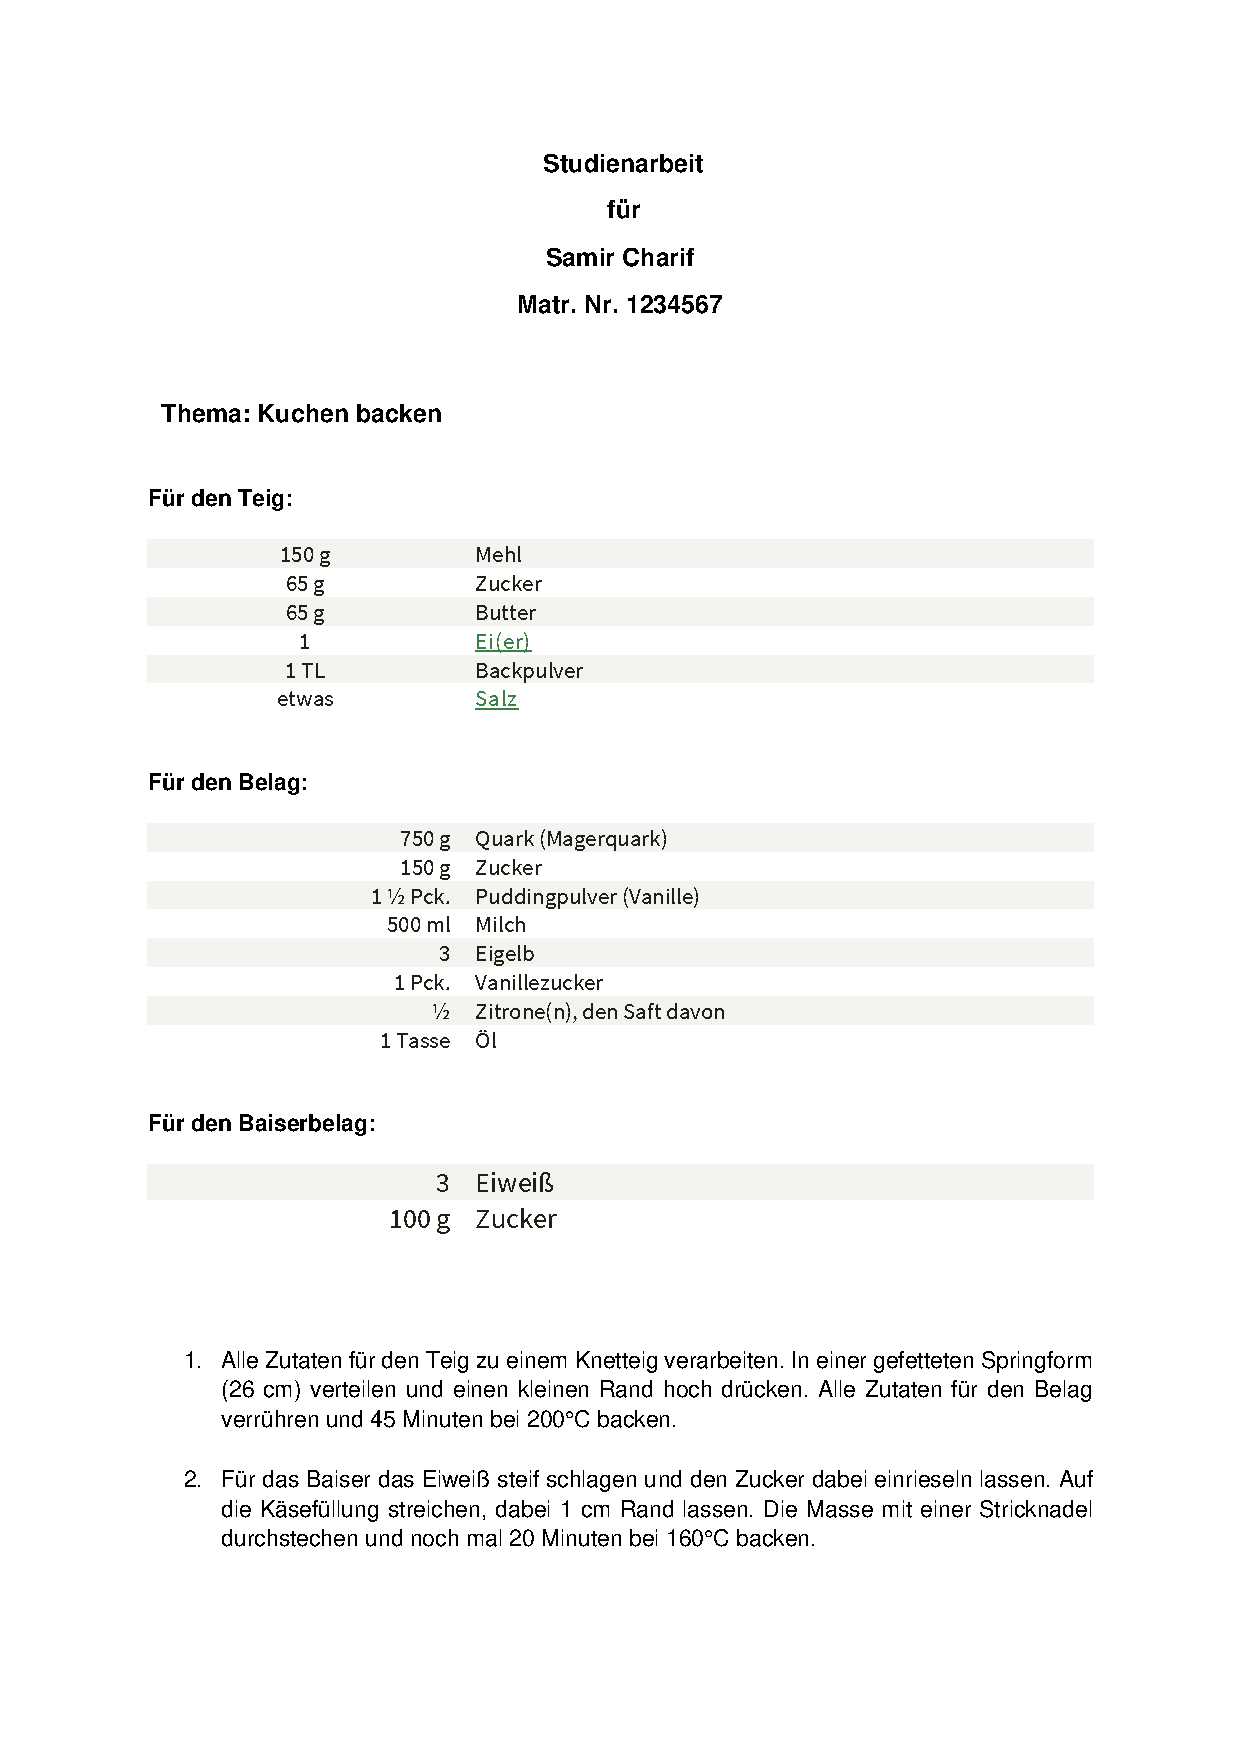
\includepdf[pages=1-]{Kapitel/Aufgabenstellung_Samir_Charif_Kuchen.pdf}
		
		%Seitenzahlen etc.
		\pagestyle{scrheadings} % Ab hier mit Kopf- und Fusszeile 
	
%	 Danksagung
	%% ++++++++++++++++++++++++++++++++++++++++++++++++++++++++++++
%% Danksagung
%% ++++++++++++++++++++++++++++++++++++++++++++++++++++++++++++
%
%  Gerüst:
%  * Version 1.0
%  * B. Ing. Samir Charif, s.charif@tu-braunschweig.de

%
%  Für Hauptseminare, Studienarbeiten, Diplomarbeiten
%
%  Autor           : Max Mustermann
%  Letzte Änderung : 04.12.2021
%
% Hier in die zweite geschweifte Klammer jeweils
% die persönlichen Daten und das Thema der Arbeit eintragen:

\section*{Danksagung}
\ldots \emph{Danksagung einfügen}\ldots


	
	% Erklärung
	%% ++++++++++++++++++++++++++++++++++++++++++++++++++++++++++++
%% Vorwort: Abschlusserklärung
%% ++++++++++++++++++++++++++++++++++++++++++++++++++++++++++++
%
%  Gerüst:
%  * Version 1.0
%  * B. Ing. Samir Charif, s.charif@tu-braunschweig.de

%
%  Für Hauptseminare, Studienarbeiten, Diplomarbeiten
%
%  Autor           : Max Mustermann
%  Letzte Änderung : 04.12.2021
%
% Hier in die zweite geschweifte Klammer jeweils
% die persönlichen Daten und das Thema der Arbeit eintragen:

\chapter*{Erklärung}
%\addcontentsline{toc}{chapter}{Erklärung}
%\ihead[]{Erklärung}
\thispagestyle{empty}
Die vorliegende Arbeit habe ich selbstständig ohne Benutzung anderer als der
angegebenen Quellen angefertigt. Alle Stellen, die wörtlich oder sinngemäß
aus veröffentlichten Quellen entnommen wurden, sind als solche
kenntlich gemacht. Die Arbeit ist in gleicher oder ähnlicher Form oder
auszugsweise im Rahmen einer oder anderer Prüfungen noch nicht vorgelegt
worden.
\\[2cm]
Braunschweig, den \hfill \namedesautors

	
%		\input{Kapitel/kurzfassung.tex}
	

	
	% Thesen (Nur bei Bedarf nutzen)
	% \input{thesen.tex}
	
	% Inhaltsverzeichnis
	\tableofcontents

		
%	 Formelzeichen Verzeichniss
	\newpage
		\printglossary[title=Nomenclature]
%	\printglossary[type=symbolslist, style=MyStyle]
	\newpage
%	

	
%	 Abbildungsverzeichnis einbinden
	\cleardoublepage
	\ihead[]{Abbildungsverzeichnis}
	\listoffigures
	
	
	% Tabellenverzeichnis einbinden
	\cleardoublepage
	\ihead[]{Tabellenverzeichnis}
	\listoftables
	\newpage
	\ihead[]{\headmark}
	
	
%
	

%	
	% Die einzelnen Kapitel
	\cleardoublepage % Seitenumbruch erzwingen vor Änderung des Nummerierungsstils
	\pagenumbering{arabic} % Nummerierung der Seiten ab hier: 1, 2, 3, 4..
	
	% Kapitel
	%  Kapitel 1:
%  * Version 1.0
%  * Samir Charif
%  * s.charif@tu-braunschweig.de
%  * Student, TU Braunschweig
%  * Mai 2022
%
\chapter{Formatierung}
\label{chap:Formatierung}

\section[Kurzer Title]{Sehr sehr sehr sehr sehr sehr sehr sehr langer Title}
\label{sec:Title}


\section{Nomenklatur}
\label{sec:nomenklatur}
Die Verwendung der einzelnen Befehle der Nomenklatur wird im Folgenden erklärt. 
Indices werden nicht kursiv geschrieben, außer es sind Laufindices. Das nicht kursiv schreiben in der Indices wird erreicht, indem bei der Erstellung eines neuen Glossaryeintrags der Befehl \verb=\mathrm{}= verwendet wird (siehe Beispieldatei).  


\begin{description}
	\item[Variable aufrufen:] \verb=\glsc{rho}= -> \glsh{rho}\\
	\verb=\glsc{mat.A}= -> \glsh{mat.A}
	% 	\item[Aufrechten Indice anfügen:] A\textbackslash sbuc\{v\} fügt aufrechten Indice an $ A\sbuc{v} A\sbu{v}$
	\item[Index] Index \verb=\glsub{mat.A}=\glsub{D}{i}
	\item[Tiefgestellt aufrecht:]  \verb=\glsub{d}{v}= -> \glsub{d}{v}.
	\item[2xTiefgestellt:]  \glsubs{D}{w}{a}, beide Indices auf gleicher Höhe.
	%	\item[2xTiefgestellt hover:] \glsubc{D}{w}, beide Indices auf gleicher Höhe.
	\item[Index anhängen] \glsvi{T}{k}
	\item[Index 2x anhängen]  \glsvisub{T}{z}{v}, Index tiefer angehängt.
	\item[Aktzente:] \glsac[dot]{m} und \glsac[bar]{T}
\end{description}

Mein Formelzeichen:   \gls{k}, \gls{mat.A} and \gls{mat.b} $\glsub{d}{v}$ 
\glsh{k} \glsac[bar]{T} \gls{rho}% \glsc{symb:R}, \glsc{symb:Re}\\

\subsection{Akronyme}
\label{subsec:akronyme}
Befehle des Glossarie Paketes:
\begin{description}
	\item[Akronym:]	 Akronyme werden beim ersten Mal ausgeschrieben \verb=\gls{ODE}= \gls{ODE}
	\item[Akronym ausgeschrieben in gewählter Sprache:] \verb=\gls{ODE}= \gls{ODE}
	\item[Akronym kurz\&klein:] \verb=\acrshort{kS}= \acrshort{kS} 
	\item[Akronym erster Buchstabe\&kurz:] \verb=\Acrshort{kS}= \Acrshort{kS} 
	\item[Akronym groß\&klein:] \verb=\ACRshort{kS}= \ACRshort{kS} 
	\item[Akronym klein\&ausgeschrieben:] \verb=\acrlong{kS}= \acrlong{kS} 
	\item[Akronym erster Buchstabe groß\&ausgeschrieben:] \verb=\Acrlong{kS}= \\ \Acrlong{kS} 
	\item[Akronym ausgeschrieben\&groß:] \verb=\ACRlong{kS}= \ACRlong{kS} 
	\item[Akronym ausgeschrieben+Abkürzung:] \verb=\acrfull{TL}= -> \acrfull{TL}
	\item[Akronym erster Buchstabe\&ausgeschrieben+Abkürzung:]\verb=\Acrfull{TL}= -> \\ \Acrfull{TL}
	\item[Akronym groß\&ausgeschrieben+Abkürzung:] \verb=\ACRfull{TL}= -> \\ \ACRfull{TL}
	\item [Akronym hover erter Aufruf:] \verb=\acfirst{TL}= -> \acfirst{TL}
	\item [Akronym benutzt hover:] \ac{TL}
\end{description}	


\subsection{SIUINTx}
\label{subsec:siunitx}
In diesem Abschnitt wird erklärt, wie das Package SIUNITX verwendet wird. Die Verwendung dieses Packages ermöglicht die Aufwandsarme und richtige Formatierung von Formeln und Einheiten. Zwischen Zahlen und Einheiten gehört ein halbes geschütztes Leerzeichen, welches mit \textbackslash, erzeugt werden kann. 

\begin{description}
	\item[Einheit:] \begin{verbatim}
		\si{\watt} = \si\{\square\metre\kilo\gram\per\cubic\second\} -> 
	\end{verbatim} 
	$\si{\watt} = \si{\square\metre\kilo\gram\per\cubic\second}$
	\item[Zahl+Einheit:] \verb=\SI{1}{\mHz} -> \SI{1}{\mHz}= \\
	\verb=\SI{1}{\mu\N}= -> \SI{1}{\mu \newton}
	\item[Exponent:] \verb=\SI{1e-4}{\meter}=	-> \SI{1e-4}{\meter}
	\item[Range:] \verb=\SIrange{1}{7}{\newton}= -> \SIrange{1}{7}{\newton}
	\item[Liste:] \verb=\SIlist{1;3;5;7}{\kN}= -> \SIlist{1;3;5;7}{\kN}
	\item[Winkel:] \verb=\ang{47;59;43}= -> \ang{47;59;43}
	\item[Fehler:] \verb=\num{9.99 +- 0.09}= -> \num{9.99 +- 0.09} 
	\item[Eigene Einheiten:] Es können eigene Einheiten deklariert werden. \\ \verb=\DeclareSIUnit\lightyear{ly} ermöglicht  \SI{1}{\lightyear}= -> \SI{1}{\lightyear}
\end{description}
Das Paket stellt zwei zusätzliche Spaltentypen S und c zur Verfügung. Wobei S für die Zahlen und s für die Einheit verwendet werden. Die Zahlen werden zentriert am Dezimalkomma beziehungsweise Punkt ausgerichtet. Die Spalte für die Einheiten (c) wird per default zentriert ausgerichtet. Sollen die Spalten für Zahlen (S) beschriftet werden, muss der Text geklammert \{Text\} werden.

\noindent
\begin{table}[H]
	\centering
	\caption[Kurz SIUNITX]{Lange Überschrift für SIUNITX}
	\begin{tabular}{l c S[table-format=10.9] S[retain-zero-exponent=true]}
		\toprule
		\multicolumn{4}{c}{SI Prefixes} \\
		\addlinespace %\midrule
		Prefix & Symbol & {Multiplication Factor} & {\dots\ in Scientific Notation} \\
		\midrule
		giga  & \siprefix{\giga} & 1000000000 & e9 \\
		mega  & \siprefix{\mega} & 1000000    & e6 \\ 
		kilo  & \siprefix{\kilo} & 1000       & e3 \\
		deca  & \siprefix{\deca} & 10         & e1 \\ % "\deka" works too
		\rowcolor{gray!20}  -- & -- & 1 & e0 \\
		deci  & \siprefix{\deci} & 0.1        & e-1 \\
		centi & \siprefix{\centi}& 0.01       & e-2 \\
		milli & \siprefix{\milli}& 0.001      & e-3 \\
		micro & \siprefix{\micro}& 0.000001   & e-6 \\
		nano  & \siprefix{\nano} & 0.000000001& e-9 \\
		\bottomrule
	\end{tabular}
\end{table}

Eine deutsche Dokumentation ist unter \href{https://www.namsu.de/Extra/pakete/Siunitx.html}{https://www.namsu.de/Extra/pakete/Siunitx.html} zu finden.
Die vollständige Dokumentation ist unter \href{https://ctan.org/pkg/siunitx?lang=de}{cta.org} zu finden. In der Originaldokumention befindet sich eine Tabelle mit weiteren kurzen Einheiten wie \textbackslash kN.


\section{Bilder}
\label{sec:bilder}

\begin{figure}[H]
	\centering
	% ---------- nomenclature base style ----------------------------------------
%\newcounter{glosmath@mainEntryCtr}% 
%\newlength{\glosmath@curNameLen}%	
%\newcommand*{\glosstyledesc}[1]{}%
% Hier eintragen welche Listen mit Einheit angezeigt werden sollen.
% Möglichkeiten: latin, greek, vecMat, subscript, operator, abbrv
\newcommand{\miteinheit}{latin, greek, vecMat}

\renewglossarystyle{glosmath@glostyle}%
{%
	\setglossarystyle{alttree}% based on alttree style
	\renewenvironment{theglossary}%
	{%
		\let\glosmath@oldparskip\parskip%
		\setlength{\parskip}{0pt}%
		\let\glosmath@oldparindent\parindent%
		\setlength{\parindent}{0pt}%
	}%
	{%
		\setlength{\parskip}{\glosmath@oldparskip}%
		\setlength{\parindent}{\glosmath@oldparindent}%
	}%
	\renewcommand*{\glossaryheader}%
	{%
		\iftoggle{glosmath@singlelineskip}{%
			\ifdefined\SingleSpacing\SingleSpacing\fi% memoir class
			\ifdefined\singlespacing\singlespacing\fi% setspace package
		}{}%
	}%
	\setcounter{glosmath@mainEntryCtr}{0}%
	\setlength{\glosmath@curNameLen}{\glstreeindent}%
	% desc in all languages of the style (default to main language only) :
	\renewcommand*{\glosstyledesc}[1]{\glsentrydesc{##1}}%
	\renewcommand*{\glossentry}[2]%
	{%
		\ifnum\value{glosmath@mainEntryCtr}>0\vspace{\baselineskip}\fi%
		\glstarget{##1}{\glscatnamefmt{\glosstyledesc{##1}}}%
		\par\nopagebreak%
		\stepcounter{glosmath@mainEntryCtr}%
	}%
	\renewcommand*{\subglossentry}[3] {%
		\IfStringInList{\glsentryparent{##2}}{\miteinheit}{%		Wenn parent = latin 
			\settowidth{\glstreeindent}{\@glswidestname\glstreepredesc}%
			\hangindent\glstreeindent%
			\settowidth{\glosmath@curNameLen}{\glossentryname{##2}\glstreepredesc}%
			% larger namebox for entries longer than @glswidestname :
			\ifdimgreater{\glosmath@curNameLen}{\glstreeindent}{%
				\setlength{\glstreeindent}{\glosmath@curNameLen}}{}%
			\glstreenamebox{\glstreeindent}{%
				\glstarget{##2}{\glossentryname{##2}}%
			}%
			\ifglshassymbol{##2}{
				\settowidth{\glstreeindent}{\@glswidestname\glstreepredesc}%
				\hangindent\glstreeindent%
				\settowidth{\glosmath@curNameLen}{\glossentrysymbol{##2}\glstreepredesc}%
				% larger namebox for entries longer than @glswidestname :
				\ifdimgreater{\glosmath@curNameLen}{\glstreeindent}{%
					\setlength{\glstreeindent}{\glosmath@curNameLen}}{}%
				\glstreenamebox{\glstreeindent}{%
					\glstarget{##2}{\glossentrysymbol{##2}}%
				}%
			}{
				\settowidth{\glstreeindent}{\@glswidestname\glstreepredesc}%
				\hangindent\glstreeindent%
				\settowidth{\glosmath@curNameLen}{\glstreepredesc}%
				% larger namebox for entries longer than @glswidestname :
				\ifdimgreater{\glosmath@curNameLen}{\glstreeindent}{%
					\setlength{\glstreeindent}{\glosmath@curNameLen}}{}%
				\glstreenamebox{\glstreeindent}{%
					\glstarget{##2}{}%
				}%
			}
			%		\ifglshassymbol{##2}{\glossentrysymbol{##2} ,\space}{}%
			\glosstyledesc{##2}%
			
			\par%
		}%
		{% else
			\settowidth{\glstreeindent}{\@glswidestname\glstreepredesc}%
			\hangindent\glstreeindent%
			\settowidth{\glosmath@curNameLen}{\glossentryname{##2}\glstreepredesc}%
			% larger namebox for entries longer than @glswidestname :
			\ifdimgreater{\glosmath@curNameLen}{\glstreeindent}{%
				\setlength{\glstreeindent}{\glosmath@curNameLen}}{}%
			\glstreenamebox{\glstreeindent}{%
				\glstarget{##2}{\glossentryname{##2}}%
			}%
			\glosstyledesc{##2}%
			
			\par%
		}%
	}%
}%


	\caption[Ü-kurz]{Test lange Überschrift}
	\label{abb:test}
\end{figure}


\section{Tabellen}
\label{sec:tabellen}

\rowcolors{1}{lightrowcolor}{white} % schöne Tabellen
\begin{table}[H]%[htb]
	\centering
	\caption[Kurz für Verzeichnis]{Randbedingungen der Längsplanung einschließlich Abtastung}
	\label{tab:rand}
	\begin{tabular}{p{4.7cm}|p{2cm}|p{2cm}|p{2cm}|p{2.3cm}}
		\rowcolor{headrowcolor}
		Parameter & Minimum & Maximum & Abtastung & Komplexität \\ \hline
		Geschwindigkeitsdifferenz & -12 & 12 & 3 & 9 \\ 
		Beschleunigung (Anfang) & -2 & 2 & 1 & 5 \\ 
		Ruck(Anfang) & -2 & 2 & 1 & 5 \\ 
		& & & & \\
		&  &  & Gesamt & 225 \\ 
	\end{tabular} 
	
	\label{tab:param_raster_laengs}
\end{table}
\rowcolors{1}{}{} % schöne Tabellen deaktivieren


\section{Quellen}
\label{sec:quellen}

Meine Quelle: 
\begin{description}
	\item[Quelle:] \verb=\cite{Dembowski.2011}= -> \cite{Dembowski.2011}
\end{description}
	\label{chap:Kapitel1}


	% Anhang mit Römischien Seitenzahlen
	\clearpage % Seitenumbruch erzwingen vor Änderung des Nummerierungsstils
	\appendix
	\pagenumbering{Roman}

	\part*{Anhang} 
	\chapter{Anhang: Expose}
	%\section[short title]{title}

\section[Problemstellung]{Problemstellung}
\label{anhang_expose:problemstellung}

\section[Fragestellung]{Fragestellung}
\label{anhang_expose:fragestellung}

\section[Ziel der Arbeit]{Ziel der Arbeit}
\label{anhang_expose:arbeitsziel}


\section[Vorgehensweise]{Vorgehensweise}
\label{anhang_expose:vorgehensweise}

	\label{chap:Expose}

	\chapter{Anhang: Aufgabenliste}
	\section[Aufgabenlise]{Aufgabenlise}
\label{anhang_aufgabenlise:Aufgabenlise}

	\label{chap:Aufgabenliste}		

	\chapter{Anhang: GanttChart}
	GanttChart Quer
	\label{chap:GanttChart}		
				
	% Literaturverzeichnis einbinden
	%% ++++++++++++++++++++++++++++++++++++++++++++++++++++++++++++
%% Anhang: Literaturverzeichnis
%% ++++++++++++++++++++++++++++++++++++++++++++++++++++++++++++
%
%  Gerüst:
%  * Version 1.0
%  * B. Ing. Samir Charif, s.charif@tu-braunschweig.de

%
%  Für Hauptseminare, Studienarbeiten, Diplomarbeiten
%
%  Autor           : Max Mustermann
%  Letzte Änderung : 04.12.2021
%
% Hier in die zweite geschweifte Klammer jeweils
% die persönlichen Daten und das Thema der Arbeit eintragen:

% Mit dem Befehl \nocite werden auch nicht im Text zitierte
% aus der Literaturdatenbank mit in das Literaturverzeichnis aufgenommen.
% Ein "\nocite{*}" übernimmt ungeprüft die komplette Datenbank.
%\nocite{*}

\cleardoublepage
\ihead[]{Literaturverzeichnis}
%\bibliographystyle{alphadin}
%\bibliography{literatur} % "literatur.bib" ist hier die einzige Literaturdatenbank.
\printbibliography
% Alternativ: Mehrere Datenbanken verwenden, falls eine
% oder mehrere umfangreiche Sammlungen exisitieren:
%\bibliography{literatur_buecher,literatur_weblinks}

	\label{chap:literaturverzeichnis}

\end{document}